\subsection{Shared-parameter verifier and operating boundaries}
The new studies address verifier choice and operating conditions separately from the complete three-block primary workloads. All prefixes, source arrays and methods are fixed before each study; every requested cutoff remains in its denominator.
\begin{table}[t]\centering\footnotesize\setlength{\tabcolsep}{3pt}
\caption{Shared-core verifier comparison, first 20 questions per graph, all 60 cutoffs. Entries are seconds / STABLE cuts. Both consume identical retained rows, tails and upward-rounded residual/resolvent bounds. SMT has a 5\,s solver limit per cutoff; all encoding time is included. One block; graph preparation and the common compiler are excluded.}
\label{tab:shared-smt}
\begin{tabular}{lrr}\toprule Graph & Bernstein & Shared SMT\\\midrule
HotpotQA & 0.683/57 & 327.87/0\\
MuSiQue & 0.118/57 & 156.19/33\\
\bottomrule\end{tabular}\end{table}
The solution-function comparator follows the shared-parameter SMT route of Junges et al.~\cite{junges2024}, implemented here with Z3 QF\_NRA rather than the PROPhESY tool. It asks whether any in-domain policy has nonpositive approximate determinant or violates a guarded selected--competitor gap, including all outside nodes through the same tails. UNSAT certifies stability; SAT only refutes this sufficient test and is not an actual instability witness. The three MuSiQue SAT cases remain UNKNOWN; the other unproved SMT cuts time out. Table~\ref{tab:shared-smt} isolates verification on the same source core; it is not an end-to-end or solver-workspace-budget-matched comparison. The SMT baseline passes an independent exact three-node positive/negative membership check.
The encoding names $D$ and all $2r$ amplitudes $F_j$, constrained to their exact monomial polynomials. Let $N_i,T_i,E,O$ be the pointwise forms of Eq.~\eqref{eq:controls}, using $|F_j|$ instead of coefficient envelopes, with $\epsilon=0$ in both verifiers. Put $L_i=N_i-T_i-2E$ and $U_i=N_i+T_i$. Within the box and polynomial equalities it checks satisfiability of
\begin{equation}
\begin{aligned}
 &(D\leq0)\ \lor\ \bigvee_{i\in T}(L_i\leq O)\\
 &\quad\lor\ \exists z:\left(\bigvee_{i\in T}L_i\leq z\right)
              \land\left(\bigvee_{j\in\mathcal C\setminus T}U_j\geq z\right).
\end{aligned}
\label{eq:smt-encoding}
\end{equation}
The threshold $z$ avoids enumerating $k(|\mathcal C|-k)$ pairs. There are $1+2r$ polynomial equalities, four box inequalities, $|\mathcal C|$ threshold inequalities and $k$ outside-gap inequalities, plus the determinant and amplitude sign tests. The 120 encodings have 597--1,967 candidates and 6,035--23,701 unique Z3 expression nodes. Each cutoff shares its named expressions internally but builds a fresh solver; there is no cross-cutoff encoding reuse. We use Z3 5.3.3 (package 5.3.3.0), \texttt{SolverFor(QF\_NRA)}, seed zero, and the logic-specific default strategy without a custom tactic. HotpotQA encoding/solve totals are 18.76/309.10\,s; MuSiQue totals are 8.11/148.08\,s. All cutoff times, constraint counts and an SMT-LIB export accompany the artifact.

\begin{table}[t]\centering\footnotesize\setlength{\tabcolsep}{2pt}
\caption{Propagation boundary on fixed first-100 prefixes, one complete paired block at each setting. Cells: complete seconds / all-cut resolved questions / UNKNOWN cutoffs. VR: Sparse; DP: fine DensePruned; Lift: compressed SourceLift. Every original prefix request remains charged.}
\label{tab:alpha-boundary}
\begin{tabular}{lrrr}\toprule Graph, $\alpha$ & VR & DP & Lift\\\midrule
Hot, 0.50 & 16.1/99/1 & 16.8/99/1 & 22.3/97/3\\
Hot, 0.85 & 38.1/99/1 & 38.8/99/1 & 49.7/99/1\\
Hot, 0.95 & 95.4/100/0 & 99.0/100/0 & 98.4/100/0\\
Mu, 0.50 & 5.2/98/2 & 5.0/98/2 & 9.4/97/3\\
Mu, 0.85 & 10.4/99/1 & 10.4/99/1 & 12.9/99/1\\
Mu, 0.95 & 23.3/100/0 & 23.0/100/0 & 29.0/100/0\\
\bottomrule\end{tabular}\end{table}
At $\alpha=.95$, both primary prefixes resolve all 100 requests. HotpotQA is near parity with compressed lifting (3.1\% lower cost in this block); MuSiQue retains 19.8\% lower cost. Figure~\ref{fig:boundary-stages} separates the increased graph-response work from audit work. These are controlled operating points, not new independent questions or three-block confidence intervals.
\begin{figure}[t]\centering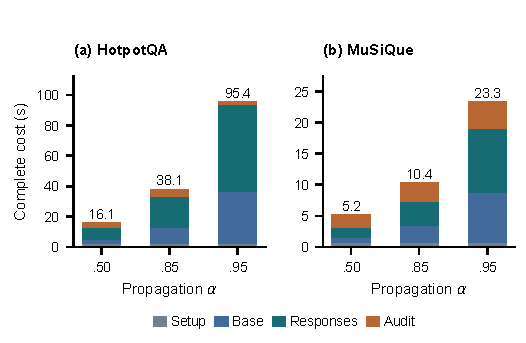
\includegraphics[width=\columnwidth]{../figures/domain_boundary_v3.pdf}
\caption{Primary complete-cost stages for Table~\ref{tab:alpha-boundary}. Base includes seed construction; Audit includes certification, actual witnesses and release; Setup includes charged startup and method setup. One complete block per setting.}
\label{fig:boundary-stages}\end{figure}
\begin{table}[t]\centering\footnotesize\setlength{\tabcolsep}{2pt}
\caption{Additional graph contexts and controlled Amazon probes; same cell format as Table~\ref{tab:alpha-boundary}. Small lexical pools use 100 queries and $\alpha=.5$. Amazon has 334,863 nodes, $\alpha=.85$, and all eight pre-existing $r=4$ seed/source requests. $+$self adds raw self weight .5 before normalization. One complete paired block; 16\,MiB admission budget.}
\label{tab:graph-boundary}
\begin{tabular}{lrrr}\toprule Graph (nodes) & VR & DP & Lift\\\midrule
Hot (9,769) & 3.9/100/0 & 3.2/100/0 & 12.0/99/1\\
Mu (12,493) & 3.3/99/1 & 3.1/99/1 & 6.4/98/2\\
Amazon & 23.7/8/0 & 40.8/3/8 & 38.0/8/0\\
Amazon +self & 22.8/8/0 & 40.4/3/8 & 38.1/8/0\\
\bottomrule\end{tabular}\end{table}
The smaller natural context pools retain their declared graph-dependent seeds/sources, so the comparison with the full pools changes graph context as well as size. Amazon uses a fixed hash-based neighbor grouping, not semantic mention links. Its zero-self original is a ratio-only control; the added-self variant exercises two policy directions. Both preserve the complete selected source arrays. The eight original $r=16$ requests are outside the current implementation\textquotesingle s $r\le4$ admission contract and receive no performance claim. Sparse resolves 8/8 in both probes, versus 3/8 for DP, and reduces complete cost against compressed lifting by 37.7\%/40.0\%. These limited probes extend execution evidence beyond the lexical topology without establishing application accuracy.
Across these ten complete cohorts, the primary's admitted numerical-state peaks span 2.98--5.79 MiB. Fresh cohort process peaks span 102.0--373.0 MiB and include all three paired method directories plus graph/backend state; they are not individual-method RSS values. Exact stage and memory records accompany the tables.
